\documentclass[conference]{IEEEtran}
\usepackage{times}
\usepackage{algorithm}
\usepackage{algpseudocode}
\usepackage{subfigure}
\usepackage{graphicx}
\usepackage{subfloat}
\usepackage{float}
\usepackage{amsmath,empheq}
\usepackage{amssymb}
\usepackage{latexsym}

\usepackage[numbers]{natbib}
\usepackage{multicol}
\usepackage[bookmarks=true]{hyperref}
\usepackage[usenames,dvipsnames]{color}
\usepackage{tikz}
\usepackage{pgfplots}

% -- Comment commands --
\newcommand{\stnote}[1]{\textcolor{Blue}{\textbf{ST: #1}}}
\newcommand{\dnote}[1]{\textcolor{Green}{\textbf{D: #1}}}
\newcommand{\enote}[1]{\textcolor{Red}{\textbf{E: #1}}}
\newcommand{\gnote}[1]{\textcolor{Purple}{\textbf{G: #1}}}

\pdfinfo{
% We'll talk about authorship when we're all together
   /Author (David Abel \& Gabriel Barth-Maron, James MacGlashan, Stefanie Tellex)
   /Title  (Toward Affordance-Aware Planning)
   /CreationDate (D:20101201120000)
   /Subject (Planning, Affordances, Sequential Decision Making)
   /Keywords (Planning, Affordance, MDP, Learning)
}

\begin{document}

% paper title
\title{Affordance-Aware Planning}

% Author info:
\author{\authorblockN{David Abel \& Gabriel Barth-Maron, James MacGlashan, Stefanie Tellex}
\authorblockA{Department of Computer Science, Brown University \\
\texttt{\{dabel,gabrielbm,jmacglashan,stefie10\}@cs.brown.edu}}}

\maketitle

\begin{abstract}
Planning algorithms for non-deterministic domains are often
intractable in large state spaces due to the well-known curse of
dimensionality. Existing approaches to planning in large stochastic state spaces fail to
prevent autonomous agents from considering many actions that are
obviously irrelevant to a human solving the same task. To solve this problem,
we formalize the notion of {\em affordances} as knowledge added to an 
Object Oriented Markov Decision Process (OO-MDP) \dnote{Should we specify the fact that
we are adding affordances to an OO-MDP in particular? Also should we note that we are goal oriented?}.
Affordances prune actions on a state-by-state basis, reducing the number of 
state-action pairs the agent must evaluate in order to behave near optimally.
% NOTE: I think it sounds punchier without this sentence, but this information might
% be important for the abstract?: (--Dave)
%Affordances are not specific to a particular reward function
%or state-space, so they may be applied to a variety of tasks and domains. 
Furthermore, we show that an agent can learn affordances through unsupervised 
experience, and that learned affordances can equal or surpass the performance of those
provided by experts. We demonstrate our approach in the state-rich Minecraft domain, 
showing significant increases in speed and reductions in state-space exploration during
planning with negligible loss in quality of the synthesized policy. Additionally, we 
employ affordance-aware planning on a robot in a collaborative cooking task. 

\end{abstract}

\IEEEpeerreviewmaketitle

% ====== Section: Introduction ======
\section{Introduction}
\label{sec:introduction}

Robots operating in unstructured, stochastic environments face
a difficult planning problem~\citep{bollini12,knepper13}.
Robotic planning tasks are classically formalized as a stochastic sequential
decision making problem, modeled as a Markov Decision Process (MDP). In these problems,
the agent must find a mapping from states to actions for some subset of the 
state space that enables the agent to achieve a goal while minimizing costs 
along the way. However, many robotics problems are of such exceeding 
complexity that modeling them as an MDP results in a massive state-action space, 
which in turn, restricts the classes of robotics problems that are computationally tractable.
 \dnote{We say "problems" a bit too often here. I tried trimming it down.}
 
For example, when a robot is manipulating objects in an environment
an object can be placed anywhere in a large set of locations. The size
of the state space increases exponentially with the number of objects,
which bounds the placement problems that the robot is able to expediently solve.

To address this state-action space explosion, prior work has explored adding knowledge to the planner,
such as options~\cite{sutton99} and macroactions~\cite{Botea:2005kx,Newton:2005vn}. 
However, while these methods allow the agent to search more deeply in the state
space, they add high-level actions to the planner which {\em increase} the size of the state-action space.
The resulting augmented space is even larger, which can have the paradoxical 
effect of increasing the search time for a good policy~\cite{Jong:2008zr}.
\dnote{Should we mention heuristic planners or action pruning work here too?}

Deterministic forward-search algorithms like hierarchical task networks (HTNs),
such as SHOP~\citep{Nau:1999:SSH:1624312.1624357}, and
temporal logical planning (TLPlan)~\citep{Bacchus95usingtemporal,Bacchus99usingtemporal}, 
add knowledge to the planner that greatly increases planning speed, but do not
generalize to stochastic domains. Additionally, the knowledge provided to the 
planner must be given by a domain expert, reducing the agent's autonomy.

To address these issues, we propose augmenting an MDP
with a formalization of {\em affordances}. An
affordance~\cite{gibson77} specifies which actions an agent should consider in
different states of the world in order to achieve its goal. By applying affordances 
to planning, we prune the agent's action set to focus on aspects of the environment
that are most relevant to solving its current goal and avoid exploration of irrelevant 
parts of the state-action space. Affordances are not specific to a particular reward
function or state space, and provide the agent with transferable knowledge that is 
effective in a wide variety of problems. Moreover, our methods enable a single agent 
to autonomously learn affordances through unsupervised experience, making affordances 
a concise, transferable, and learnable means of representing useful planning knowledge.

%% Because affordances define the {\em kind} of goals for which actions
%% are useful, affordances also enable high-level reasoning that can be
%% combined with approaches like subgoal planning for even
%% greater performance gains. 

Our experiments demonstrate that affordances provide dramatic speedups for a variety
of planning tasks compared to baselines and apply across different state-spaces.  We 
conduct experiments in the game Minecraft, and on a robotic cooking assistant. 

% ====== Background ======
\section{Background}
\label{sec:background}
% --- Subsection: MDPS ---
%\subsection{MDPs}
A classic MDP is a five-tuple: $\langle \mathcal{S}, \mathcal{A}, \mathcal{T},
\mathcal{R}, \gamma \rangle$, where $\mathcal{S}$ is a state-space;
$\mathcal{A}$ is the agent's set of actions; $\mathcal{T}$ denotes
$\mathcal{T}(s' \mid s,a)$, the transition probability of an agent
applying action $a \in \mathcal{A}$ in state $s \in \mathcal{S}$ and
arriving in $s' \in \mathcal{S}$; $\mathcal{R}(s,a,s')$ denotes the
reward received by the agent for applying action $a$ in state $s$ and
and transitioning to state $s'$; and $\gamma \in [0, 1)$ is a discount
factor that defines how much the agent prefers immediate rewards
over distant rewards (the agent prefers to maximize
immediate rewards as $\gamma$ decreases). A classic way to 
provide a factored representation of an MDP state is to represent
each MDP state as a single feature vector. 

% -- Subsection: OO-MDPs --
\subsection{OO-MDPs}
An Object-Oriented Markov
Decision Process (OO-MDP)~\citep{diuk08} can be used to represent an MDP.
Unlike the vectorized state of an MDP, an OO-MDP state is a collection of objects,
$O = \{o_1, \ldots, o_o \}$.  Each object $o_i$ belongs to a
class, $c_j \in  \{c_1, \ldots, c_c\}$. Every class has a set of attributes,
$Att(c) = \{c.a_1, \ldots, c.a_a \}$, each of which has a domain, $Dom(c.a)$, of 
possible values. The collection of attribute values of a given object is termed 
that object's state, $o.state$. A vectorized MDP state can be equivalently understood as the set
of all the object states, $s \in {\cal S} = \cup_{i = 1}^o \{o_i.state\}$, in an OO-MDP. 


%% An OO-MDP lies in the ability to
%% formulate predicates over classes of objects. That is, the OO-MDP
%% definition also includes a set of predicates ${\cal P}$ that operate
%% on the state of objects to provide additional high-level information
%% about the MDP state. 

%% While an OO-MDP reduces the size of the state space by a significant
%% factor, the resulting state space is still far too large to solve with
%% any existing (OO)-MDP solver. This is the primary motivator for
%% incorporating affordances - to reduce the amount of the state space
%% that an OO-MDP agent will have to explore.

%% The Brown UMBC Reinforcement Learning And Planning framework (BURLAP\footnote{http://burlap.cs.brown.edu/})
%% is working toward integrating planning and reinforcement learning algorithms with a variety of planning domains represented
%% as an OO-MDP, including ROS. In this way, transferable knowledge like affordances can be quickly deployed
%% to domains like Mountain Car \cite{Moore90efficientmemory-based} and Minecraft, but also to a variety
%% of Robots that utilize ROS. Our group is also working to deploy affordances as a
%% means of knowledge representation and reasoning for collaborative cooking with ReThink's Baxter.


% ====== Section: Affordances ======
\section{Affordances}
\label{sec:affordances}

The term ``affordance" was introduced by J.J. Gibson in 1977~\citep{gibson77}. An 
affordance describes the action-possibilities that an environment presents to an agent.
More specifically, Gibson proposed that an affordance is ``what [the environment] offers
[an] animal, what [the environment] provides or furnishes, either for good or ill".
\dnote{I moved MDPs and OO-MDPs into the "background" section, and added a brief affordance intro here - thoughts? MDPs/OO-MDPs felt odd at the beginning of the affordances section}

% -- Subsection: Affordance Formalism --
\subsection{Affordance Formalism}

\enote{we need to fix this formalism as per what we talked about Dave -- i.e. it's an object or a mapping...}
\dnote{Ellis how about this? It's a little weird for the mapping to utilize elements of the tuple, but I think this
paints the right picture. My other thought would be to replace M and n with alpha and beta, where they act as hyper params for
the Dirichlet-multinomial and Dirichlet, respectively. That allows the formalism to tie more directly into the learning.}

% -- "Equation": Affordance Formalism --
 We define an affordance, $\Delta$, as the tuple $\langle p, g, \delta, \alpha, \beta \rangle$,
where:
\begin{itemize}
\item $p$ is a predicate on states, $s \longrightarrow \{$0$, 1\}$ representing the {\em precondition} for the affordance. 
\item $g$ is a {\it goal type}, representing the type of problem the agent is solving.
\item $\delta$ is a mapping from an OO-MDP state $s$ and a goal type $G$ to a set of actions $A \subset \mathcal{A}$.
\item $\alpha$ is a vector of counts of each action.
\item $\beta$ is a vector of counts of the integers from 1 to $|\mathcal{A}|$, where $\mathcal{A}$ is the action set of the OO-MDP.
\end{itemize}

The precondition, $p$, and goal type, $g$, refer to predicates that are defined in the OO-MDP definition.
The precondition specifies when certain affordances are relevant, and the goal allows the agent to focus
on different actions depending on what it is trying to accomplish. The mapping $\delta$
represents a function that determines the relevant action possibilities for the affordance in each state:

% -- Equation: Delta mapping --
\begin{equation}
\delta(s,G)= 
\begin{cases}
    A, & \text{if } \Delta.p(s) \wedge G \models \Delta.g \\
    \varnothing,              & \text{otherwise}
\end{cases}
\label{eq:delta_mapping}
\end{equation}

\dnote{There must be a more concise way of phrasing this.. Realistically we want delta to {\it return} a sample from a Dirichlet-multinomial distribution with alpha as the hyper parameter, and n as the set size, where n is a sample from a Dirichlet with beta as the hyper parameter. This description works but it forces the introduction of $A$ which seems unnecessary. There is ``experiment" notation from cryptography, but I don't think that is widely used outside of the field?}

We define the set of actions contributed by the affordance, $A$, to be the result
of taking $n$ samples (without replacement) from a multinomial over the OO-MDP
action space. We model this sampling with a Dirichlet-multinomial distribution:

% -- Equation: Dirichlet-multinomail sampling --
\begin{equation} 
\begin{split}
n &\sim Dir(\Delta.\beta) \\
A &\leftarrow DirMult(\Delta.\alpha, n)
\end{split}
\label{eq:dir_mult_sample}
\end{equation}
\dnote{Should we make these variables affordance specific? I.e.: $n \sim Dir(\Delta_j.\beta)$, and $A \leftarrow DirMult(\alpha,n)$.}

Where $\Delta.\alpha$ is the hyper parameter of action counts, $n$ is sampled 
from a Dirichlet distribution over action set sizes with $\beta$ as the hyper parameter
of action set size counts. Provided that the hyper parameters associated with each 
affordance are properly specified, the probability of retrieving the optimal action set 
across all affordances, as seen in Equation \ref{eq:opt}, approaches 1 as the counts 
of $\alpha$ and $\beta$ approach the optimal counts. Properly setting these counts 
is a difficult problem, however, which is why the learning problem is non-trivial.

Our definition of affordances builds on OO-MDPs. Using OO-MDP predicates for affordance
preconditions and goal types allows for state space independence, as predicates generalize across state-spaces. 
\enote{I think a sentence explaining/emphasizing this would be good since it's not entirely obvious at a first pass why OO-MDPs give you state-space independence}. \dnote{I added a note here but it sounds superfluous to me. Let me know what you think} 
Thus, a planner equipped with affordances can be used in any number of
different environments. For instance, the affordances defined for navigation problems 
can be used in any task regardless of the spatial size of the world, number of objects in 
the world, and specific goal the agent is trying to satisfy.

% -- Subsection: Affordance-Aware Planning --
\subsection{Affordance-Aware Planning}
Affordances restrict the action set of a planner on a state by state basis. 
Namely, for each state, the planner's available actions are set to be the 
union of all action sets provided by all affordances, $\mathcal{A}_{\Delta}$, 
which is a subset of the full action set $\mathcal{A}$. 

% -- Equation: Affordance Union --
\begin{align}
\mathcal{A}_{\Delta} = \left(\bigcup\limits_{j = 1}^{|\Delta|} \Delta_j.\delta(s,G) \right) \subseteq \mathcal{A}
\label{eq:afford_union}
\end{align}

Any OO-MDP solver may be made affordance-aware by replacing the 
OO-MDP's action set $\mathcal{A}$ in each state with the affordance 
suggested action set $\mathcal{A}_\Delta$. If $\mathcal{A}_\Delta$ is 
ever empty, the planner uses the full OO-MDP action set.

Our goal is that the set of affordance actions, $\mathcal{A}_{\Delta}$, 
is equal to the set of optimal actions, $\mathcal{A}^o$ for a given state:

% --- Equation: Master---
\begin{equation} 
\Pr( \mathcal{A}_{\Delta} = \mathcal{A}^o \mid s, G, \Delta_1 \dots \Delta_K) = 1
\label{eq:opt}
\end{equation}

This probability can be equivalently understood as the probability that each
optimal action is in $\mathcal{A}_{\Delta}$ and each non-optimal action is 
not in $\mathcal{A}_{\Delta}$:

% -- Equation: Is in optimal, is not in non-optimal --
\begin{multline}
= \left[\prod_i^{|\mathcal{A}^o|} \sum_j^{|\Delta|} \Pr(a_i \in \Delta_j.\delta(s,G) \mid s, G, \Delta_j)\right] \\
\times \left[1 - \prod_i^{|\overline{\mathcal{A}^o}|} \sum_j^{|\Delta|} \Pr(b_i \in \Delta_j.\delta(s,G) \mid s, G, \Delta_j)\right]
\label{eq:isin_notin}
\end{multline}

Where $a_i$ is an optimal action for the given state, $a_i \in \mathcal{A}^o$,
and $b_i$ is a non-optimal action for the given state, $b_i \in \overline{\mathcal{A}^o}$.
Equation \ref{eq:isin_notin} represents the probability that each optimal action is in the
affordance action set, and that each non-optimal action is not in the affordance action set.

A domain expert may specify the hyper parameters $\alpha$ and $\beta$ directly,
allowing $\mathcal{A_\Delta}$ to be computed deterministically in the limit if 
the expert desires. If an expert is not involved, the agent learns $\alpha$ and
$\beta$ for each affordance during training time. Note that $\Pr(a_i \in \Delta_j.\delta(s,G) \mid s, \Delta_j)$ is
defined as the probability that the given action $a_i$ is in a sample from the Dirichlet-multinomial
in Equation~\ref{eq:dir_mult_sample}.

% --- Subsection: Learning Affordances ---
\subsection{Learning Affordances}

Even with expert domain knowledge it is often unclear how to create
an optimal knowledge base, and it can be arduous to specify a 
large number of affordances. We developed an unsupervised learning
process that requires only minimal seeding from an expert.
The full learning algorithm is shown in Algorithm~\ref{alg:learn}.

To learn an affordance knowledge base, a domain 
expert must supply a set of relevant domain specific predicates,
$\mathcal{P}$ and possible goals the agent will have to solve, $\mathcal{G}
\subset \mathcal{P}$. Additionally, a domain expert must provide a means 
of generating candidate state spaces in which each goal $g \in \mathcal{G}$
may be satisfied (i.e. the function $createTestWorld(g)$ at line 5 in Algorithm \ref{alg:learn}).

% -- Algorithm: Learning ---
\begin{algorithm}
  \caption{$learn(\mathcal{P}, \mathcal{G})$}
  \begin{algorithmic}[1]
    \For {$(p, g) \in \mathcal{P} \times \mathcal{G}$}
    \State $knowledgeBase.add(\Delta(p,g))$
    \EndFor
    \For {$g \in \mathcal{G}$}
    \State $w_i = createTestWorld(g)$
    \State $\pi_i = planner.solve(w_i, g)$
    \State $updateParameters(knowledgeBase, \pi_i)$
    \EndFor
    \State $removeLowInfoAffordances(knowledgeBase)$
  \end{algorithmic}
  \label{alg:learn}
\end{algorithm}

The primary tasks in learning affordances is to learn reasonable precondition-goal 
combinations, and to learn $\alpha$ and $\beta$ for each affordance. 

To determine good $p$ and $g$ pairs, the algorithm creates one affordance for 
each combination of $\langle p, g \rangle$, where $p \in \mathcal{P}$ and $g
\in \mathcal{G}$, as seen in line 1-3 of Algorithm \ref{alg:learn}. Affordances
whose precondition-goal pairs don't provide useful information are thrown out 
by the function call on line 9, leaving only those affordances with sound 
precondition-goal pairs. We chose to remove affordances with little or no $\alpha$
counts at the end of training, or those whose $\alpha$ counts were close to the 
actual action distribution of the policy, indicating that the affordance contained little 
information.

To learn the $\alpha$ and $\beta$ for each
affordance, we synthesize a policy of $m$ goal-annotated
OO-MDPs that have small state spaces, but share similar characteristics
to more complex state spaces the agent might expect to see at test time.
For example, the agent learns to build bridges over trenches in small state
spaces that can be solved exactly (i.e. a state space of several thousand states), but
generalizes its knowledge to worlds that are too large to solve with exact algorithms
(state spaces of hundreds of thousands of states). With this policy, we know the optimal 
action in each state and can generalize this optimality to larger state spaces.

% -- Algorithm: Update Parameters --
\begin{algorithm}
  \caption{$updateParameters(knowledgeBase, \pi)$}
  \begin{algorithmic}[1]
    \For {$state \in \pi.reachableStates()$}
    \For {$\Delta \in knowledgeBase$}
    \If	{$\Delta.p(s) \wedge \Delta.g \models s.g$}
    \State $\Delta.\alpha(\pi.getOptimalAction(s))$++
    \EndIf
    \EndFor
    \EndFor
  \end{algorithmic}
  \label{alg:update_params}
  \caption{\dnote{I need to add beta counts to this algorithm. It's a bit tricky to do concisely so I'm taking some time on it}}
\end{algorithm}

We update $\alpha$ and $\beta$ according to Algorithm~\ref{lag:update_params}.
For each optimal policy, for each affordance, $\alpha$ is set to the number of states
in which an action was optimal when its affordance's predicate was true and goal was
entailed by the present goal. Additionally, we count the number of unique actions that
were optimal for each activated affordance $\Delta_i$, and increment that value for
$\Delta_i.\beta$.\dnote{Does this make sense?} This captures how large or small optimal
action sets are expected to be for each affordance.

% ====== Section: Experiments ======
\section{Experiments}
\label{sec:experiments}

We use Minecraft as our planning and evaluation domain. Minecraft is a
3-D blocks game in which the user can place, craft, and destroy blocks
of different types. It serves as a model for a variety of complex planning tasks involving 
assembly, crafting, and construction.  Minecraft's physics and action space are expressive
enough to allow users to create complex systems, including logic gates and 
functional scientific graphing calculators\footnote{https://www.youtube.com/watch?v=wgJfVRhotlQ}.
Minecraft serves as a model for robotic tasks such as cooking assistance, assembling
items in a factory, object retrieval, and complex terrain traversal.  As in these tasks, 
the agent operates in a very large state-action space in an uncertain environment.

For experiments, we introduce a simplified baseline version of the affordance where
the action set $A$ associated computed by $\Delta.\delta$ is defined
as the set of actions whose probability of being optimal was greater than $1\%$
of the probability mass of the multinomial created over the $\alpha$ counts. This
baseline is listed as $LT$ (for learned threshold).

% -- Subsection: Minecraft Tests --
\subsection{Minecraft Tests}
We conducted a series of experiments in the Minecraft domain that
compared the performance of several planner without affordances
to their affordance-aware counterparts. We created a set of expert
affordances from our background knowledge of the domain, which are
listed in Figure \ref{fig:afford_kb_exp}. Additionally, we ran our full
learning process and learned affordances for each task. We compared
standard paradigm planners (Real Time Dynamic Programming and 
Value Iteration) with their expert-affordance-aware counterparts and with
their learned-affordance-aware counterparts.

% -- Figure: List of expert affordances used --
\begin{figure}
Figure listing the expert affordances
\label{fig:afford_kb_exp}
\end{figure}

Our experiments consisted of 5 common tasks in Minecraft, including
constructing bridges over trenches, smelting gold, tunneling
through walls, and digging to find an object.  We tested on 
randomized worlds of varying size and difficulty. The generated test
worlds varied in size from tens of thousands of states to hundreds of thousands of states.

The training data consisted of 10 simple state spaces of each map type
(50 total), each approximately a 1,000-10,000 state world with randomized
features that mirrored the agent's actual state space. The same training data
was used for each test state space.

The evaluation metric for each trial was the
number of Bellman updates that were executed by each planning
algorithm, as well as the CPU time taken to find a plan. Value Iteration
was terminated when the maximum change in the value function was 
less than 0.01. RTDP was terminated when the maximum change in 
the value function was less than 0.01 for fifty consecutive policy rollouts,
or the planner failed to converge after 2500 rollouts. We set the reward 
function to $-1$ for all transitions, except transitions to states in which 
the agent was on lava, which returned $-10$. The goal was set to be 
terminal. The discount factor was set to $\lambda = 0.99$. For all experiments,
movement actions (move, rotate, jump) had a small probability (0.05) of 
incorrectly applying a different movement action.

% -- Subsection: Learning Rate --
\subsection{Learning Rate}
\dnote{Note: the metric has been changed from number of worlds to number of
states (which is really the important number)} Additionally, we conducted 
experiments in which we varied the number of states visited at training time. 
As in Table \ref{table:learned-results}, we randomly generated simple state spaces
containing several thousand states containing features that mirrored the agent's state
space at test time. We then solved the OO-MDP with knowledge bases learned from 
10 to 10000 states.

% -- Subsection: Temporally Extended Actions --
\subsection{Temporally Extended Actions}
Furthermore, we compared our approach to Temporally Extended Actions: 
macroactions and options. We compared RTDP with expert affordances, 
expert Macroactions, and expert Options, as well as the combination of 
affordances, macroactions, and options. We conducted these experiments 
with the same configurations as our Minecraft experiments. The option policies
and macro actions provided were hand coded by domain experts.

% -- Subsection: Robotic Task --
\subsection{Robotic Task}
Finally, we deployed an affordance-aware planner onto Baxter for use
in an assistive cooking task. \dnote{Need to fill in more details here}

% ====== Section: Results ======
\section{Results}
\label{sec:results}

% -- Subsection: Baxter --
\subsection{Baxter}

% -- Figure: Baxter results/image
\begin{figure}[H]
\centering
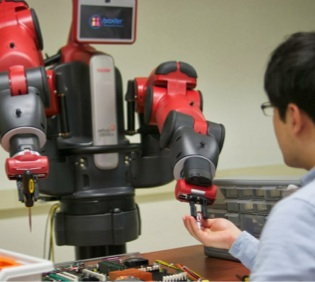
\includegraphics[scale=0.195]{figures/baxter_temp.jpg}%
  \caption{Placeholder for baxter results/image}
  \label{fig:baxter_results}
\end{figure}

% -- Subsection: Minecraft --
\subsection{Minecraft: Expert vs Learned vs None}

\dnote{Result tables will be replaced with bar charts.}

% -- Figure: Minecraft results, RTDP --
\begin{table}[H]
\centering
\begin{tabular}{ l  l || c c c c }
  State Space 		&	Size 	&	RTDP 	& Learned 	& Learned Threshold & Expert 	\\ \hline
  \texttt{Trench}  	& 	-	&	-	&	-		&	-	&	-	\\
  \texttt{Mine}  		& 	-	&	-	&	-		&	-   	&	-	\\
  \texttt{Smelt}  		& 	-	&	-	&	-		&	-	&	-	\\
  \texttt{Wall}  		& 	-	&	-	&	-		&	-	&	-	\\
  \texttt{Plane}  		& 	-	&	-	&	-		&	- 	&	-	\\
\end{tabular}
\caption{Place holder for RTDP Bellman/CPU}
\label{table:minecraft_results_bellman}
\end{table}

% -- Figure: Minecraft results, VI --
\begin{table}[H]
\centering
\begin{tabular}{ l l || c c c c }
  State Space 		&	Size 	&	RTDP 	& Learned & Learned Threshold & Expert 	\\ \hline
  \texttt{Trench}  	& 	-	&	-		&	-	&	-			&	-	\\
  \texttt{Mine}  		& 	-	&	-		&	-	&	-  			&	-	\\
  \texttt{Smelt}  		& 	-	&	-		&	-	&	-  			&	-	\\
  \texttt{Wall}  		& 	-	&	-		&	-	&	-			&	-	\\
  \texttt{Climb}  		& 	-	&	-		&	-	&	- 			&	-	\\
\end{tabular}
\caption{Place holder for VI Bellman/CPU}
\label{table:minecraft_results_bellman}
\end{table}

% -- Subsection: Minecraft Learning Rate
\subsection{Minecraft: Learning rate}

% -- Figure: Learning rate results --
\begin{figure}[H]
\centering
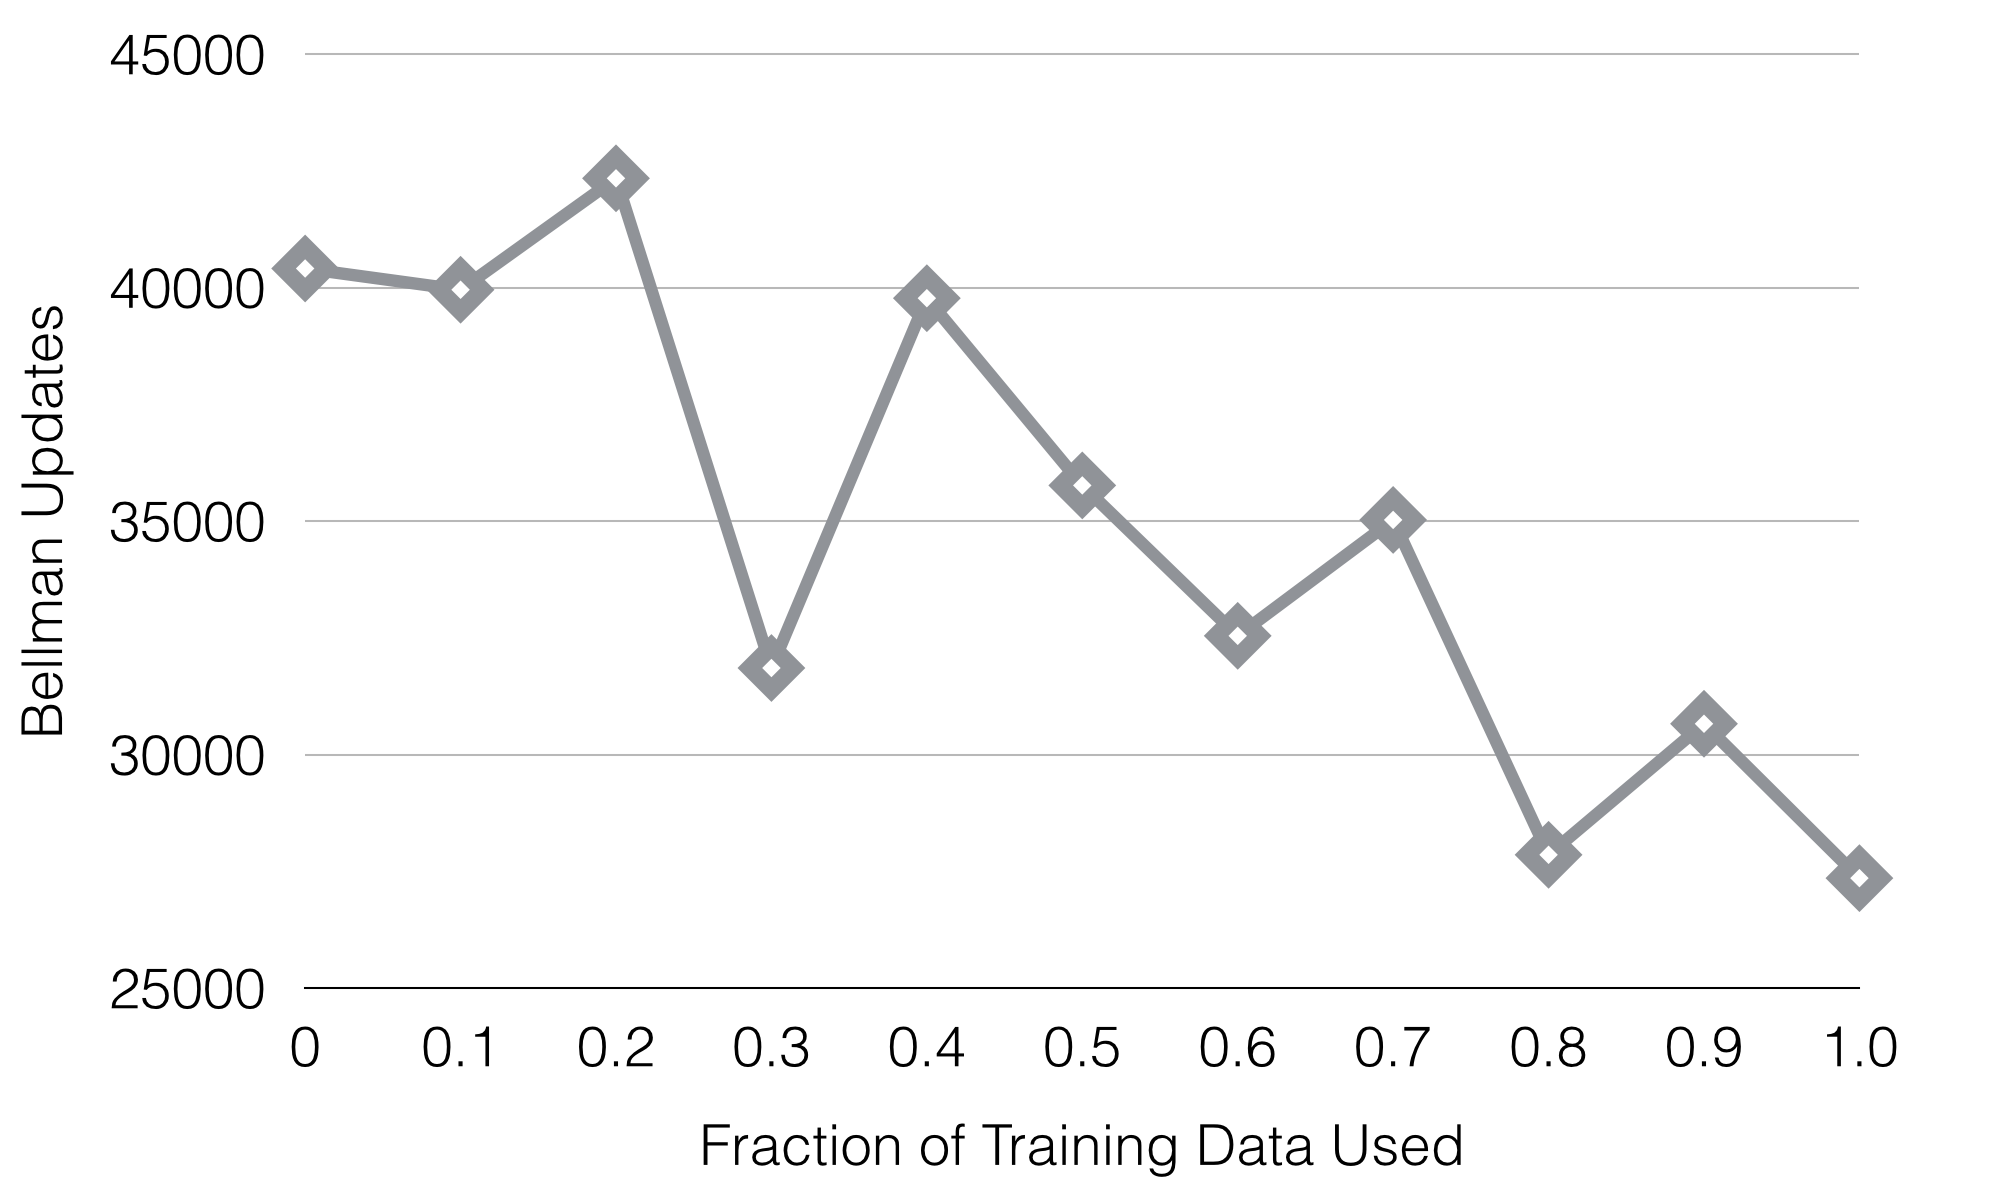
\includegraphics[scale=0.195]{figures/training_results.png}%
  \caption{Place holder for learning rate results}
  \label{fig:training_results}
\end{figure}

% -- Subsection: Temporally Extended Actions --
\subsection{Temporally Extended Actions}

% -- Figure: Options Results --
\begin{table}[H]
\centering
\begin{tabular}{ l l || c c c c }
  State Space 		&	Size 	&	Options 	& Macroactions & Affordances  & 	All 	\\ \hline
  \texttt{Trench}  	& 	-	&	-		&	-	&	-			&	-	\\
  \texttt{Mine}  		& 	-	&	-		&	-	&	-  			&	-	\\
  \texttt{Smelt}  		& 	-	&	-		&	-	&	-  			&	-	\\
  \texttt{Wall}  		& 	-	&	-		&	-	&	-			&	-	\\
  \texttt{Climb}  		& 	-	&	-		&	-	&	- 			&	-	\\
\end{tabular}
\caption{Placeholder: Temporally Extended Actions vs Affordances}
\label{table:minecraft_results_cpu}
\end{table}

% ====== Section: Related Work ======
\section{Related Work}
\label{sec:related-work}

In this section, we discuss the differences between
affordance-aware planning and other forms of knowledge engineering that
have been used to accelerate planning. We divide these approaches
into those that are built to plan in stochastic domains, and those that are
deterministic planners.

% -- Subsection: Stochastic --
\subsection{Stochastic Approaches}

% --- Subsection: Temporally Extended Actions ---
\subsubsection{Temporally Extended Actions}
Temporally extended actions are actions that the agent can
select like any other action of the domain, except executing them
results in multiple primitive actions being executed in
succession. Two common forms of temporally extended actions are {\em
  macro-actions}~\cite{hauskrecht98} ~and {\em options}~\cite{sutton99}. 
Macro-actions are actions that always
execute the same sequence of primitive actions. Options are defined
with high-level policies that accomplish specific sub tasks. For
instance, when an agent is near a door, the agent can engage the
`door-opening-option-policy', which switches from the standard
high-level planner to running a policy that is hand crafted to open
doors. 

Although the classic options framework is not generalizable to different state spaces,
creating {\em portable} options is a topic of active research~\cite{konidaris07,konidaris2009efficient,Ravindran03analgebraic,croonenborghs2008learning,andre2002state,konidaris2012transfer}.

Given the potential for unhelpful temporally extended actions to negatively impact planning time~\cite{Jong:2008zr}, we believe combing affordances with temporally extended actions
may be especially valuable because it will restrict the set of temporally extended actions to those
useful for a task. We conducted a set of experiments to investigate this intuition.

% --- Subsection: Action Pruning ---
\subsubsection{Action Pruning}

Sherstov and Stone~\cite{sherstov2005improving} considered MDPs with a very large 
action set and for which the action set of the optimal policy of a source task could be 
transferred to a new, but similar, target task to reduce the learning time required to find
the optimal policy in the target task. The main difference between our affordance-based 
action set pruning and this action transfer work is that affordances prune away actions on 
a state by state basis, where as the learned action pruning is on per task level. Further, 
with lifted goal descriptions, affordances may be attached to subgoal planning for a significant
benefit in planning tasks where complete subgoal knowledge is known.

Rosman and Ramamoorthy~\cite{rosman2012good} provide a method for learning action
priors over a set of related tasks. Specifically, they compute a Dirichlet distribution over 
actions by extracting the frequency that each action was optimal in each state for each 
previously solved task.

There are a few limitations of the actions priors work that affordance-aware planning
does not possess: (1) the action priors can only be used with planning/learning algorithms
that work well with an $\epsilon$-greedy rollout policy; (2) the priors are only utilized for 
fraction $\epsilon$ of the time steps, which is typically quite small; and (3) as variance in
tasks explored increases, the priors will become more uniform. In contrast, affordance-aware
planning can be used in a wide range of planning algorithms, benefits from the pruned action
set in every time step, and the affordance defined lifted goal-description enables higher-level 
reasoning such as subgoal planning.

% --- Subsubsection: Heuristics ---
\subsubsection{Heuristics}
Heuristics in MDPs are used to convey information about the value of a given state-action pair with respect to the task being solved and typically take the form of either {\em value function initialization},
or {\em reward shaping}. Initializing the value function to an admissible close approximation of the optimal value function has been shown to be effective for LAO* and RTDP~\cite{Hansen:1999qf}.

Reward shaping is an alternative approach to providing heuristics. The planning algorithm uses a modified version of the reward function that returns larger rewards for state-action pairs that are expected to be useful, but does not guarantee convergence to an optimal policy unless certain properties of the shaped reward are satisfied~\cite{potshap}.

A critical difference between heuristics and affordances is that heuristics are highly dependent on the reward function and state space of the task being solved, whereas affordances are state space independent and transferable between different reward functions. However, if a heuristic can be provided, the combination of heuristics and affordances may even more greatly accelerate planning algorithms than either approach alone.

% -- Subsection: Deterministic knowledge engineering approaches --
\subsection{Deterministic Approaches}

There have been several successful attempts at engineering knowledge to
decrease planning time for deterministic planners. These are fundamentally solving
a different problem from what we are interested in, but there approaches are interesting to consider.
\dnote{Need to rephrase this with justification for dealing with deterministic planners}.

% --- Subsubsection: Hierarchical Task Networks ---
\subsubsection{Hierarchical Task Networks}

\dnote{I think we should have a shoutout to Branavan's Learning High Level Plans from Text paper in this section (and include subgoal planning as part of this section}

\enote{I've been writing traditional as I expect we'll discover some HTNs that grapple with the issues stated below -- which we should probably cite}Traditional Hierarchical Task Networks (HTNs) employ \textit{task decompositions} to aid in planning. The goal at hand is decomposed into smaller tasks which are in turn decomposed into smaller tasks. This decomposition continues until primitive tasks that are immediately achievable are derived. The current state of the task decomposition, in turn, informs constraints which reduce the space over which the planner searches.

At a high level both HTNs and affordances fulfill the same role: both achieve action pruning by exploiting some form of supplied knowledge. HTNs do so with the use of information regarding both the task decomposition of the goal at hand and the sorts constraints that said decomposition imposes upon the planner. Similarly, affordances require knowledge as to how to extract values for propositional functions of interest by querying the state.

However there are three of essential distinctions between affordances and traditional HTNs. (1) HTNs deal exclusively with deterministic domains as opposed to the stochastic spaces with which affordances grapple. As a result they produce plans and not policies. (2) Moreover, HTNs do not incorporate reward into their planning. Consequently, they lack mathematical guarantees of optimal planning. \enote{I think.. We should double check this.} (3) On a qualitative level, the degree of supplied knowledge in HTNs surpasses that of affordances: whereas affordances simply require relevant propositional functions, HTNs require not only constraints for sub-tasks but a hierarchical framework of arbitrary complexity. Thus, despite a superficial similarity between affordances and HTNs wherein both employ supplied knowledge, the two deal with disparate forms of planning problems; HTN's planning problem is deterministic, reward-agnostic and necessitates a plethora of knowledge while affordances solve a planning problem that is stochastic, reward-aware and requires only relatively basic knowledge about the domain.
\enote{Need citations for HTNs}
\dnote{needs to be shorter}
% --- Subsubsection: Temporal Logic ---
\subsubsection{Temporal Logic}

Bacchus and Kabanza~\cite{Bacchus95usingtemporal,Bacchus99usingtemporal} provided
planners with domain dependent knowledge in the form of a first-order version of linear
temporal logic (LTL), which they used for control of a forward-chaining planner. With this methodology, 
a \textsc{Strips} style planner may be guided through the search space by checking 
whether candidate plans do not falsify a given knowledge base of LTL formulas, often
achieving polynomial time planning in exponential space.

The primary difference between this body of work and affordance-aware planning is that affordances may be learned (increasing autonomy of the agent), while LTL formulas are far too complicated to learn effectively, placing dependence on an expert.

% ====== Section: Conclusion ======
\section{Conclusion}
\label{sec:conclusion}
\dnote{Conclusion could use some work/rewriting}
We proposed a novel approach to representing transferable knowledge in terms of
{\em affordances}~\cite{gibson77} that allows an agent to efficiently prune actions 
based on domain knowledge, providing a significant reduction in the number of state-action
pairs the agent needs to evaluate in order to act near optimally. We demonstrated the 
effectiveness of the affordance model by comparing standard planners to their affordance-aware
equivalents in a series of challenging planning tasks in the Minecraft domain. Further, we designed
a full learning process that allows an agent to autonomously learn useful affordances that may be used
across a variety of task types, reward functions, and state-spaces, allowing for convenient extensions 
to robotic applications.

We compared the effectiveness of augmenting planners with affordances compared to 
temporally extended actions. The results suggest that affordances, when combined with 
temporally extended actions, provide substantial reduction in the portion of the state-action 
space that needs to be explored.

Lastly, we deployed an affordance-aware planner on a robotic task with a massive 
state space. \dnote{Need to flesh out once we have more detail}.

In the future, we hope to automatically discover useful state-space-specific-subgoals online 
- a topic of some active research \cite{Mcgovern01automaticdiscovery,Simsek:2005:IUS:1102351.1102454}.
This will allow for affordances to plug into high-level subgoal planning, which will reduce the size of the 
explored state-action space and improve the relevance of the action pruning. Additionally, we hope to 
decrease the amount of knowledge given to the planner by implementing lowering the expert seed 
requirements for learning affordances. One plan is to only provide a base of primitive predicates, and 
to implement Incremental Feature Dependency Discovery ~\cite{ICML2011Geramifard_473}, allowing 
our affordance learning algorithm to discover novel preconditions that will further enhance action pruning.
\dnote{Maybe put in a note about the forward search sparse sampling algorithm? Or perhaps the Bayesian planner?}

{\small
\bibliographystyle{plainnat}
\bibliography{main}
}
\end{document}


